\documentclass{article}

\usepackage[left=2cm,right=2cm,top=2cm,bottom=2cm]{geometry} 

\usepackage[utf8]{inputenc}   % otra alternativa para los caracteres acentuados y la "ñ"
\usepackage[           spanish % para poder usar el español
                      ,es-tabla % para los captions de las tablas
                       ]{babel}   
\decimalpoint %para usar el punto decimal en vez de coma para los números con decimales

%\usepackage{beton}
%\usepackage[T1]{fontenc}

\usepackage{parskip}
\usepackage{xcolor}

\usepackage{booktabs,longtable,array}
\newcolumntype{L}[1]{>{\raggedright\let\newline\\\arraybackslash\hspace{0pt}}m{#1}}
\newcolumntype{C}[1]{>{\centering\let\newline\\\arraybackslash\hspace{0pt}}m{#1}}
\newcolumntype{R}[1]{>{\raggedleft\let\newline\\\arraybackslash\hspace{0pt}}m{#1}}

\usepackage{caption}

\usepackage{enumerate} % paquete para poder personalizar fácilmente la apariencia de las listas enumerativas

\usepackage{graphicx} % figuras
\usepackage{subfigure} % subfiguras

\usepackage{amsfonts}
\usepackage{amsmath}

\usepackage{colortbl}

\usepackage{listings}
\lstset
{ %Formatting for code in appendix
    language=python,
    basicstyle=\footnotesize,
    stepnumber=1,
    showstringspaces=false,
    tabsize=1,
    breaklines=true,
    breakatwhitespace=false,
}

\definecolor{softpink}{rgb}{1,0.8,1}
	
\usepackage{float} % para controlar la situación de los entornos flotantes

\restylefloat{figure}
\restylefloat{table} 
\setlength{\parindent}{0mm}


\usepackage[bookmarks=true,
            bookmarksnumbered=false, % true means bookmarks in 
                                     % left window are numbered
            bookmarksopen=false,     % true means only level 1
                                     % are displayed.
            colorlinks=true,
            allcolors=blue,
            urlcolor=blue]{hyperref}
\definecolor{webblue}{rgb}{0, 0, 0.5}  % less intense blue

\renewcommand{\thesection}{\arabic{section}}

\title{\Huge Inteligencia de Negocio: Práctica 3 \\ Competición de Kaggle\vspace{10mm}}

\author{\huge David Cabezas Berrido \vspace{10mm} \\ 
  \huge Grupo 2: Viernes \vspace{10mm} \\ \huge dxabezas@correo.ugr.es \vspace{10mm}}

\begin{document}
\maketitle

\pagebreak

\begin{figure}[H]
  \centering
  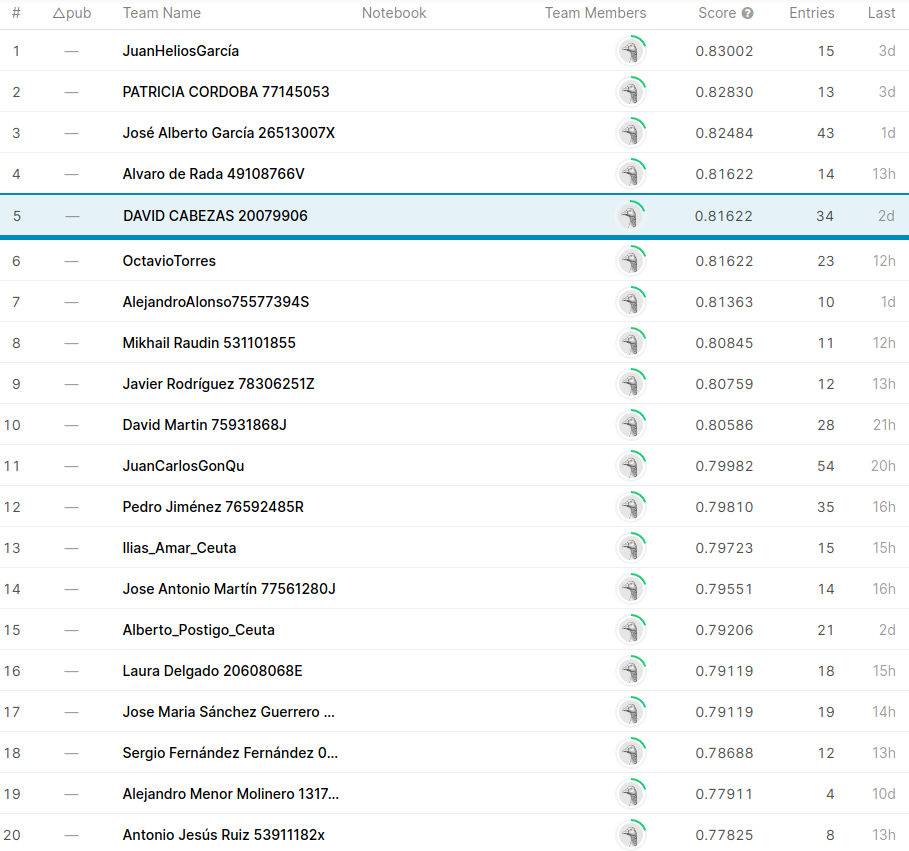
\includegraphics[width=180mm]{leaderboard}
  \caption{Leaderboard definitiva de la competición.}
  \label{fig:leaderboard}
\end{figure}

\pagebreak

\tableofcontents

\pagebreak

\section{Pruebas realizadas}
\setlength\LTleft{-0.5in}
\setlength\LTright{-2in}
\begin{longtable}{|c|C{2.1cm}|c|c|c|C{4cm}|C{6cm}|}
\toprule
Intento & Fecha-hora & Posición & Validación & Test & Preprocesado & Modelo \\

\midrule

1 & 19/12/2020 14:35:08 & 5 & 0.8185 & 0.7420 & Preprocesado 1 & RandomForest por defecto \\

\arrayrulecolor{black!10}\midrule

2 & 20/12/2020 10:51:19 & 4-5 & 0.8900 & 0.7580 & Preprocesado 2 & RandomForest por defecto \\

\arrayrulecolor{black!10}\midrule

3 & 20/12/2020 12:34:18 & 4-5 & 0.9040 & 0.7498 & Preprocesado 2 eliminando de train los ejemplos que inicialmente tenían descuento & RandomForest con 350 estimadores de profundidad máxima 20 \\

\arrayrulecolor{black!10}\midrule

4 & 20/12/2020 17:05:16 & 3-4 & 0.9179 & 0.7645 & Preprocesado 3 & MLPClassifier con capas ocultas de tamaño (200,200) \\

\arrayrulecolor{black!10}\midrule

5 & 21/12/2020 09:47:11 & 3-4 & 0.8750 & 0.6877 & Preprocesado 3 & 2-NN con distancia Manhattan y pesos inversamente proporcionales a la distancia \\

\arrayrulecolor{black!10}\midrule

6 & 21/12/2020 13:30:36 & 3 & 0.9143 & 0.7739 & Preprocesado 3 & C-SVM con C=65 y kernel RBF \\

\arrayrulecolor{black!10}\midrule

7 & 21/12/2020 15:32:20 & 3 & 0.9144 & 0.7645 & Preprocesado 3 & RandomForest por defecto \\

\arrayrulecolor{black!10}\midrule

8 & 22/12/2020 09:49:44 & 2 & 0.9143 & 0.8059 & Preprocesado 3 & GradientBoosting con 500 estimadores \\

\arrayrulecolor{black!10}\midrule

9 & 22/12/2020 09:50:03 & 2 & 0.9304 & 0.8016 & Preprocesado 3 & Stacking: - RandomForest por defecto - MLPClassifier con capas ocultas (200,200) - C-SVM con C=65 y kernel RBF - GradientBoosting con 500 estimadores \\

\arrayrulecolor{black!10}\midrule

10 & 22/12/2020 14:40:39 & 2 & 0.9312 & 0.7636 & Preprocesado 3 & AdaBoost con 500 árboles de profundidad 12 y learning rate de 1.1 \\

\arrayrulecolor{black!10}\midrule

11 & 23/12/2020 10:24:20 & 2 & 0.9163 & 0.7990 & Preprocesado 3 sustituyendo los valores perdidos por 0 en la columna descuento en lugar de eliminar la columna & GradientBoosting con 500 estimadores \\

\arrayrulecolor{black!10}\midrule

12 & 23/12/2020 12:12:38 & 2 &  & 0.7998 & Preprocesado 3 & Moda (predicción más frecuente) de los intentos 4, 6, 7, 8, 9, 10 y 11 \\

\arrayrulecolor{black!10}\midrule

13 & 24/12/2020 19:54:10 & 2 & 0.9205 & 0.7886 & Preprocesado 3 & GradientBoosting con 500 árboles de profundidad 6, learning rate de 1.175 y submuestras del 70\% \\

\arrayrulecolor{black!10}\midrule

14 & 25/12/2020 09:59:17 & 4 & 0.8535 & 0.7239 & Preprocesado 3 + PCA con 0.95 de varianza explicada & GradientBoosting con 500 estimadores \\

\arrayrulecolor{black!10}\midrule

15 & 25/12/2020 10:25:21 & 4 & 0.9159 & 0.8007 & Preprocesado 3 tras corregir error en LabelEncoder & GradientBoosting con 500 estimadores \\

\arrayrulecolor{black!10}\midrule

16 & 25/12/2020 11:33:44 & 4 &  & 0.8093 & Preprocesado 3 & Stacking de cuatro GradientBoosting con número de estimadores 450, 500, 550 y 600 respectivamente; tasas de aprendizaje 0.14, 0.12, 0.1, 0.08 respectivamente; todos con submuestras del 90\% \\

\arrayrulecolor{black!10}\midrule

17 & 26/12/2020 10:58:03 & 4 &  & 0.8085 & Preprocesado 3 & Stacking anterior con la opción passthrough \\

\arrayrulecolor{black!10}\midrule

18 & 26/12/2020 11:12:21 & 4 & 0.9268  & 0.7886 & Preprocesado 3 & HistGradientBoosting por defecto \\

\arrayrulecolor{black!10}\midrule

19 & 26/12/2020 11:31:13 & 4 & & 0.8024 & Preprocesado 3 & Stacking de tres
GradientBoosting con 500, 550 y 600 estimadores respectivamente; tasas
de aprendizaje 0.12, 0.1 y 0.08 respectivamente; todos con submuestras
del 90\%. También tres HistGradientBoosting con 100, 150 y 200 iteraciones máximas respectivamente \\

\arrayrulecolor{black!10}\midrule

20 & 27/12/2020 11:00:35 & 4 &  & 0.8016 & Preprocesado 3 & Stacking de cuatro GradientBoosting con número de estimadores 450, 500, 550 y 600 respectivamente; tasas de aprendizaje 0.14, 0.12, 0.1, 0.08 respectivamente; todos con submuestras del 90\%. También dos HistGradientBoosting con 100 y 200 iteraciones máximas respectivamente \\

\arrayrulecolor{black!10}\midrule

21 & 27/12/2020 13:54:7 & 4 & (0.8392) & 0.7886 & Preprocesado 3 & GradientBoosting con 550 árboles de profundidad 2, tasa de aprendizaje de 0.15 y submuestras del 90\% \\

\arrayrulecolor{black!10}\midrule

22 & 27/12/2020 14:30:41 & 4 & (0.8462) & 0.7790 & Preprocesado 3 & LightGBM con 125 árboles de profundidad máxima 8 y 27 nodos hoja como máximo; tasa de aprendizaje del 0.08 \\

\arrayrulecolor{black!10}\midrule

23 & 28/12/2020 09:21:46 & 4 & 0.9290 & 0.7808 & Preprocesado 3 & LightGBM con 200 árboles con profundiad máxima 14 \\

\arrayrulecolor{black!10}\midrule

24 & 28/12/2020 09:22:13 & 4 & 0.9291 & 0.7843 & Preprocesado 3 & LightGBM con 125 árboles con 29 nodos hoja como máximo; tasa de aprendizaje del 0.11 \\

\arrayrulecolor{black!10}\midrule

25 & 28/12/2020 09:16:14 & 4 & 0.9266 & 0.7817 & Preprocesado 3 & LightGBM por defecto \\

\arrayrulecolor{black!10}\midrule

26 & 29/12/2020 10:42:25 & 4 & \begin{tabular}[c]{c} (0.8151) \\ 0.8990  \end{tabular} & 0.7964 & Preprocesado 3 & MLP con early stopping \\

\arrayrulecolor{black!10}\midrule

27 & 29/12/2020 10:52:45 & 4 & \begin{tabular}[c]{c} (0.7920) \\ 0.9135  \end{tabular}  & 0.778 & Preprocesado 3 & SVM con C=40 \\

\arrayrulecolor{black!10}\midrule

28 & 29/12/2020 13:27:51 & 4 & \begin{tabular}[c]{c} (0.8352) \\ 0.9207 \end{tabular}  & 0.8016 & Preprocesado 3 & XGBoost con 200 árboles de profundidad 3 \\

\arrayrulecolor{black!10}\midrule

29 & 30/12/2020 09:45:53 & 4 & \begin{tabular}[c]{c} (0.8370) \\ 0.9262  \end{tabular}  & 0.7929 & Preprocesado 3 & HistGradientBoosting con 75 iteraciones máximas \\

\arrayrulecolor{black!10}\midrule

30 & 30/12/2020 09:43:11 & 4 & 0.9300  & 0.7774 & Preprocesado 3 & HistGradientBoosting con 200 iteraciones máximas, tasa de aprendizaje del 0.08 y árboles con 29 nodos hoja como máximo \\

\arrayrulecolor{black!10}\midrule

31 & 30/12/2020 10:08:35 & 4 & 0.9304  & 0.8110 & Preprocesado 3 & Stacking de GradientBoosting con 500 estimadores, MLP con early stopping, XGBoost con 200 árboles de profundidad 3 y HistGradientBoosting con 75 iteraciones máximas \\

\arrayrulecolor{black!10}\midrule

\rowcolor{softpink}

32 & 31/12/2020 10:14:38 & 5 & 0.9268  & 0.8162 & Preprocesado 3 & Stacking de GradientBoosting con 500 estimadores, MLP con early stopping y XGBoost con 200 árboles de profundidad 3 \\

\arrayrulecolor{black!10}\midrule

33 & 31/12/2020 11:29:18 & 5 & 0.9225  & 0.8067 & Preprocesado 3 & Stacking de GradientBoosting con 500 estimadores y y XGBoost con 200 árboles de profundidad 3 \\

\arrayrulecolor{black}\bottomrule
\caption{Pruebas realizadas}
\label{tab:pruebas}
\end{longtable}

\textbf{Nota:} Los valores entre paréntesis en la columna de
validación no corresponden a validación cruzada, sino a un conjunto de
validación que he separado para paliar un problema de sobreajuste. Ver Sección \ref{val-sobreajuste}.

\textbf{Nota 2:} El intento $n$, corresponde al archivo
\texttt{try$n$.csv}, pero en Kaggle corresponde al $n+1$ debido a que
subí un intento corrupto por un error en el formato de la salida.

\pagebreak

\section{Introducción}

TODO

\pagebreak

\section{Preprocesados}

El número de datos que presentaban valores perdidos en alguna de las
columnas era bastante bajo, del orden de pocos cientos entre los cerca
de 4800 datos, y no hay valores perdidos en los datos de test; es por
ello que desechamos las instancias con valores perdidos en alguna de
las columnas. Una excepción es la columna Descuento, en la que la gran
mayoría de las instancias carecen de valor, por esta razón tomamos la
decisión de desechar la columna. Hablaremos sobre ella más tarde.

Una vez tratado el problema de los valores perdidos, probamos distintas técnicas de preprocesado.

El \textbf{Preprocesado 1} es el mínimo para que os algoritmos puedan
ejecutarse. Codificamos las variables categóricas con
\texttt{LabelEncoder}, primero nos quedamos con la marca del coche, ya
que hay cerca de 2000 modelos y son demasiados para que los algoritmos
puedan aprovechar la información sólo con los algo más de 4000 datos
de entrenamiento de los que disponemos. Convertimos Consumo, Motor\_CC
y Potencia a numérica: por ejemplo, el string \texttt{23.4 kmpl} se
convierte en el flotante 23.4. También codificamos la mano como
numérica (del 1 al 4).

Con este procesamiento sólo hemos probado el intento 1, seguidamente
intentamos mejorarlo.

Las clases están desbalanceadas, hay una (3) con casi la mitad de las
instancias de entrenamiento y otras con cerca del 5\% de las
instancias. Para balancearlas he probado dos técnicas que se nos
explicaron en el seminario sobre balanceo. La primera ha sido
undersampling, y la deseché por obtener resultados bastante peores con
Random Forest por defecto que el preprocesado 1. La segunda ha sido
oversampling con \texttt{SMOTE}, que corresponde al
\textbf{Preprocesado 2}. Esta técnica si ha supuesto una mejora
significativa y he decidido mantenerla. Con este preprocesamiento,
sólo he probado los intentos 2 y 3, éste último con una modificación que comentaremos en la Sección \ref{descuento}.

El \textbf{Preprocesado 3} aplica técnicas que acostumbran a
beneficiar a modelos como KNN, SVM y redes neuronales. Estas técnicas
son la binarización de características nominales y la estandarización
de los datos (reescalarlos y desplazarlos para que tengan media 0 y
varianza 1). He mantenido este preprocesamiento por el resto de
experimentos, añadiendo pequeñas variaciones en el intento 11
(relativa a la columna Descuento) y en el intento 14, en el que he
combinado este preprocesamiento con PCA para el 95\% de variabilidad
explicada, pero resultados peores.

En el intento 15, he corregido un error en el código que enumeraba
incorrectamente los valores de la columna Mano (el 1 debe corresponder
a primera mano, el 2 a segunda, el 3 a tercera y el 4 a cuarta o
más). También he aprovechado para eliminar la única instancia de
entrenamiento correspondiente a un coche eléctrico, ya que el conjunto
de test no presenta instancias correspondientes a este tipo de
coches. Todos los intentos posteriores se realizan con la nueva
versión corregida de este preprocesamiento, aunque no parece que el
error tuviese poca relevancia (de hecho el intento 15 obtiene peor
score en test que el 8, correspondiente al mismo modelo sin el arreglo
en los datos).

\pagebreak

\section{Estimación de hiperparámetros}

\subsection{Sobreajuste con oversampling y validación
  cruzada} \label{val-sobreajuste}

\pagebreak

\section{Modelos}

\pagebreak

\section{Otras pruebas fallidas}

Describo otras estrategias que he intentado pero desechado por obtener
scores bastante bajos en validación.

\subsection{Experimentos con la columna descuento} \label{descuento}

\subsection{Naive-Bayes}

\subsection{Clustering}

\section{Webgrafía}

\end{document}
